\chapter{TINJAUAN PUSTAKA}
\label{chap:tinjauanpustaka}

\section{Penelitian Terkait}
\label{sec:penelitianTerkait}

% Contoh input gambar
\begin{figure}[H]
  \centering

  % Ubah dengan nama file gambar dan ukuran yang akan digunakan
  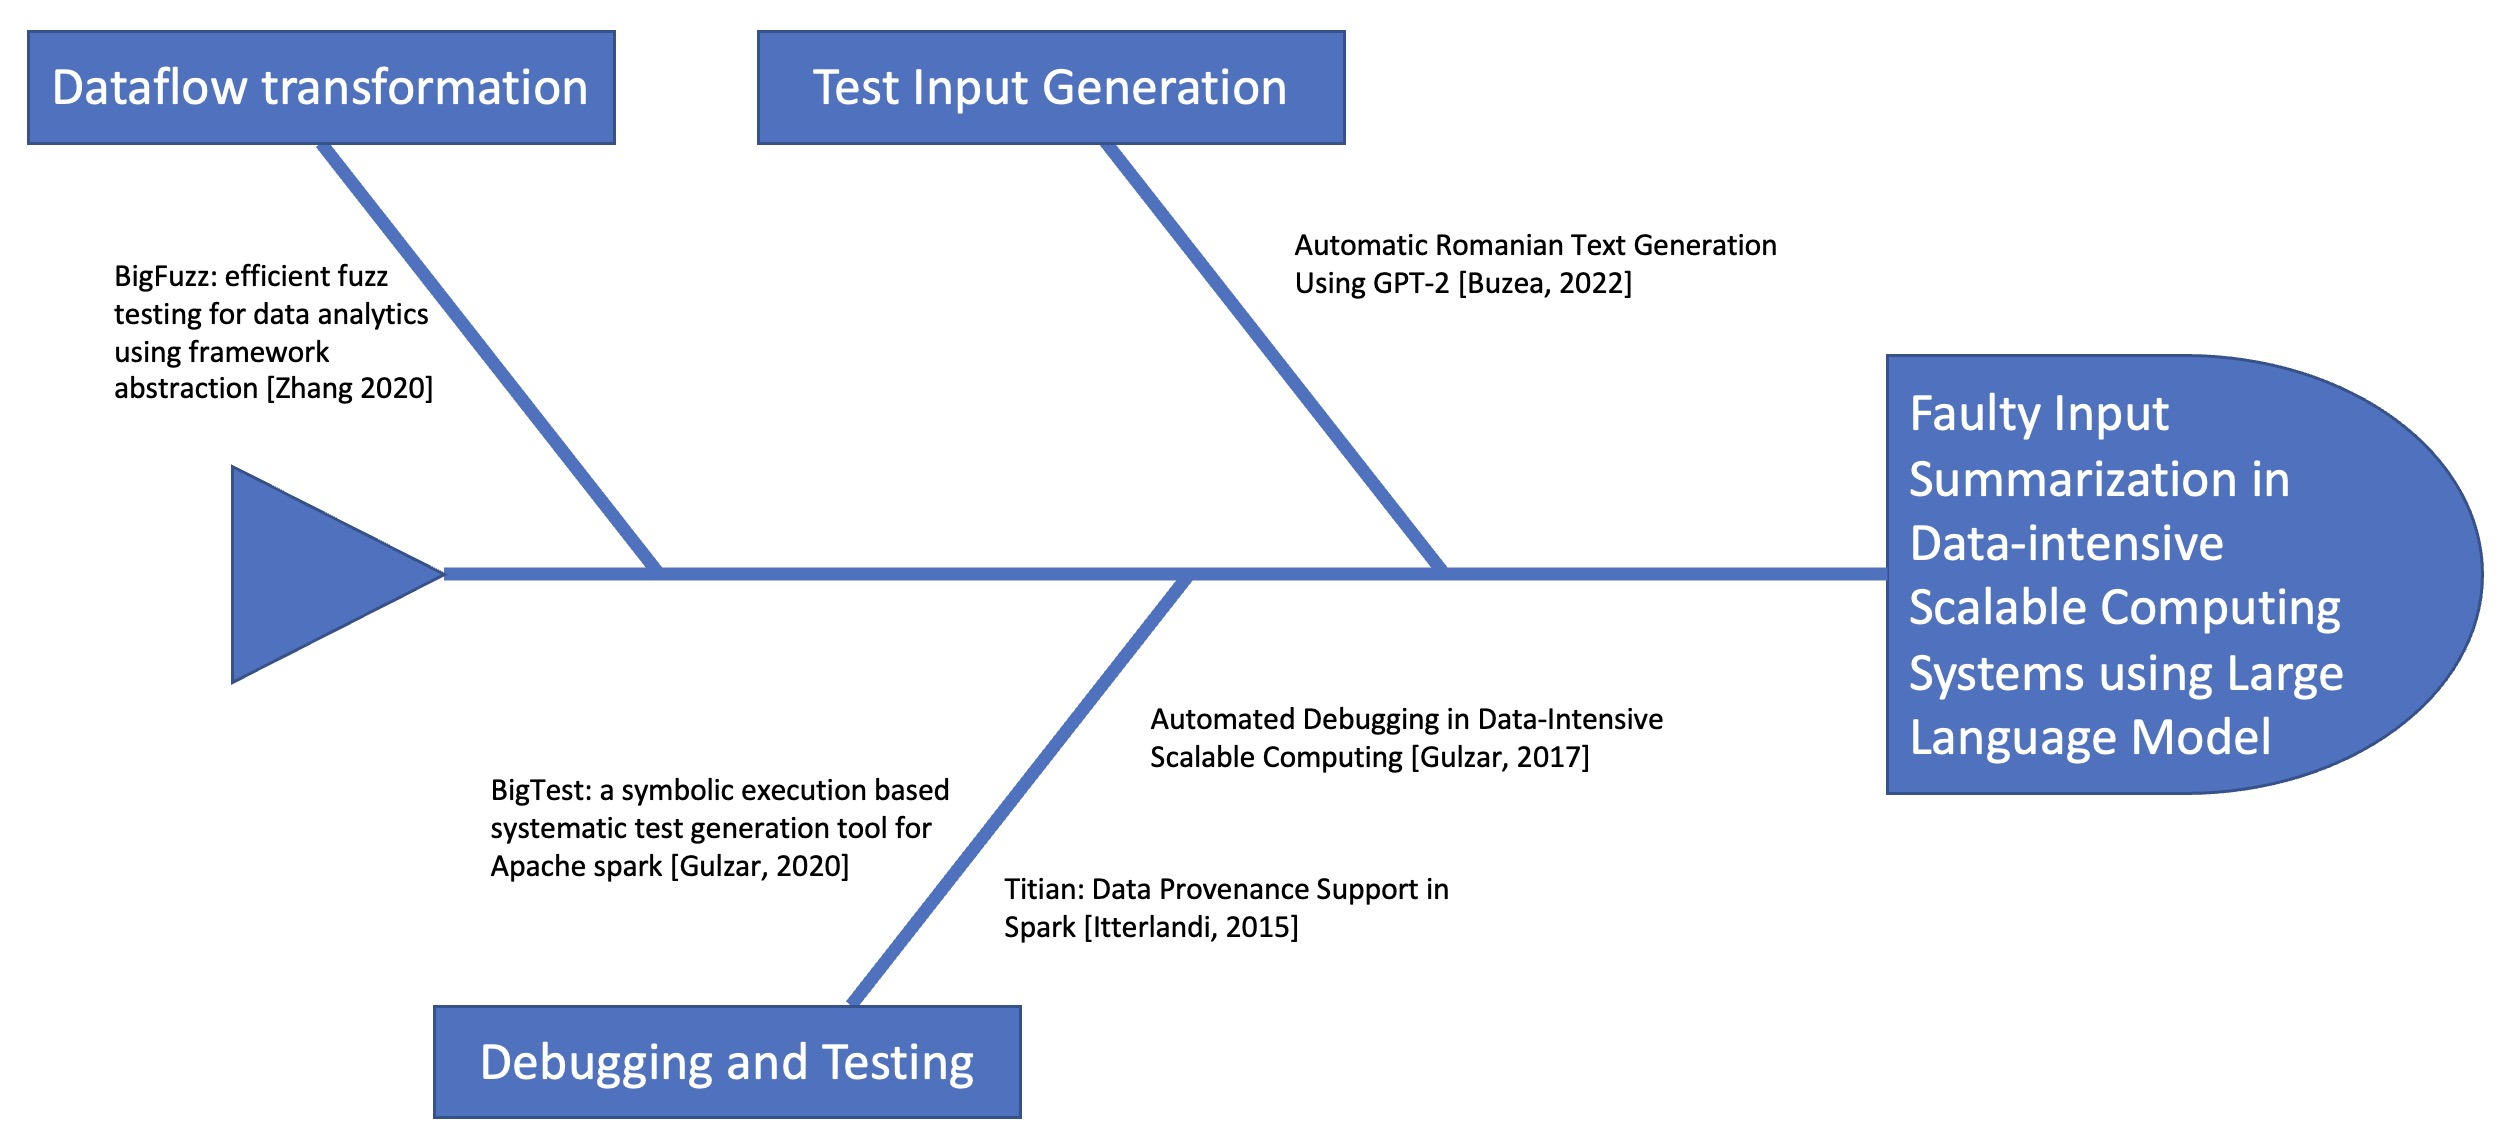
\includegraphics[scale=0.17]{gambar/StateOfTheArt.jpg}

  % Ubah dengan keterangan gambar yang diinginkan
  \caption{Diagram \emph{Fishbone}}
  \label{fig:fishbone}
\end{figure}

\subsection{\emph{Automated Debugging in Data-Intensive Scalable Computing}}
\label{subsec:Automated Debugging in Data-Intensive Scalable Computing}

Penelitian yang dilakukan oleh Muhammad Ali Gulzar dan rekan-rekannya fokus pada pengembangan beban kerja \emph{Big Data Analytics}. Mereka menghadapi tantangan dalam \emph{debugging}, terutama terkait dengan data tidak terstruktur dan asumsi yang salah mengenai data, yang sering menyebabkan kesalahan dalam program. Untuk mengatasi masalah ini, penelitian ini memperkenalkan metode baru yang disebut BIGSIFT, yang berfokus pada menemukan lokasi data yang menyebabkan kegagalan. Metode yang digunakan yaitu menggabungkan isolasi kesalahan otomatis dalam rekayasa perangkat lunak dengan \emph{provenans} data dalam sistem basis data. Hasil dari penelitian ini adalah peningkatan drastis dalam akurasi dalam menentukan lokasi kesalahan, dengan hasil yang lebih akurat hingga ribuan hingga jutaan kali lipat dibandingkan dengan metode sebelumnya seperti provenans data Titian dan \emph{Delta Debugging}. Dengan demikian, penelitian ini berpotensi memberikan manfaat besar dalam mempercepat proses \emph{debugging} pada beban kerja \emph{Big Data Analytics}, sehingga pengembang dapat mengidentifikasi dan memperbaiki masalah lebih efisien.

\subsection{\emph{BigFuzz: Efficient Fuzz Testing for Data Analytics Using Framework Abstraction}}
\label{subsec:BigFuzz: Efficient Fuzz Testing for Data Analytics Using Framework Abstraction}

Dalam penelitian yang dilakukan oleh Qian Zhang dan timnya, mereka mengatasi tantangan dalam pengujian otomatis untuk sistem data-intensive scalable computing (DISC), yang sangat penting untuk menangani kumpulan data besar dalam konteks analisis big data. Masalah utamanya terletak pada kompleksitas intrinsik dari aplikasi berbasis data semacam itu, di mana data seringkali tidak lengkap, terus berubah, dan sulit untuk diprediksi. Pengujian \emph{fuzzing} tradisional, meskipun efektif di domain lain seperti keamanan, menghadapi hambatan yang signifikan ketika diterapkan langsung pada analisis big data. Alasannya termasuk lamanya latensi sistem DISC, tidak praktisnya cakupan cabang konvensional, dan kesulitan dalam menghasilkan data yang bermakna dengan mutasi acak. Untuk mengatasi tantangan ini, para peneliti mengusulkan alat pengujian \emph{fuzzing} yang dipandu cakupan yang baru untuk analisis big data, yang disebut BigFuzz. Alat ini berfokus pada pengujian logika aplikasi daripada peningkatan cakupan kode kerangka kerja, dengan mengabstraksi kerangka kerja DISC menggunakan spesifikasi. BigFuzz juga menggunakan operator \emph{schema-aware data mutation} berdasarkan analisis mendalam tentang jenis kesalahan aplikasi DISC. Hasil penelitian menunjukkan bahwa BigFuzz secara signifikan mempercepat proses \emph{fuzzing}, meningkatkan cakupan kode, dan meningkatkan deteksi kesalahan dalam aplikasi DISC, menjadikannya alat berharga untuk \emph{debugging} beban kerja analisis \emph{big data}, dapat diterapkan pada beragam program, dan mampu menemukan lebih banyak kesalahan dibandingkan dengan pendekatan terkini yang menggunakan eksekusi simbolik.

\subsection{\emph{BigTest: A Symbolic Execution Based Systematic Test Generation Tool for Apache Spark}}
\label{subsec:BigTest: A Symbolic Execution Based Systematic Test Generation Tool for Apache Spark}

Muhammad Ali Gulzar dan timnya melakukan penelitian dalam bidang sistem komputasi berbasis data yang besar (DISC), seperti MapReduce milik Google, Apache Hadoop, dan Apache Spark, yang digunakan luas dalam layanan produksi. Meskipun aplikasi DISC sangat populer, seringkali kualitas aplikasinya kurang baik karena kurangnya pengujian yang menyeluruh dan otomatis. Saat ini, pengujian aplikasi DISC biasanya hanya menggunakan contoh kecil acak dari data masukan, yang mungkin tidak cukup untuk menemukan masalah dalam program. Pengujian aplikasi DISC memiliki tantangan tersendiri karena menggabungkan operasi aliran data dan relasional, serta fungsi yang bisa sangat kompleks.Untuk mengatasi masalah ini, para peneliti memperkenalkan kerangka pengujian putih yang baru bernama BigTest. BigTest digunakan untuk program Apache Spark dan secara otomatis menghasilkan data buatan untuk pengujian yang efektif dan efisien. BigTest menggabungkan eksekusi simbolik fungsi pengguna dengan spesifikasi logis operasi aliran data dan relasional untuk mengeksplorasi semua jalur dalam aplikasi DISC. Hasil eksperimen menunjukkan bahwa BigTest mampu menemukan dua kali lipat lebih banyak masalah daripada menggunakan seluruh dataset dengan waktu pengujian yang jauh lebih singkat (194 kali lebih cepat). BigTest diimplementasikan sebagai alat baris perintah berbasis Java dengan file biner pra-kompilasi. Pengguna dapat menyesuaikan preferensi melalui file konfigurasi, termasuk program target, batasan eksplorasi \emph{loop}, dan pemilihan penyelesaian teorema. Penelitian ini berpotensi meningkatkan pengujian aplikasi DISC, sehingga masalah dalam program dapat ditemukan dengan lebih efektif dan efisien.

\subsection{\emph{Titian: Data Provenance Support in Spark}}
\label{subsec:Titian: Data Provenance Support in Spark}

Matteo Itterlandi dan timnya mengatasi tantangan yang sulit dalam melakukan \emph{debugging} pada logika pemrosesan data di dalam sistem Data-Intensive Scalable Computing (DISC). Biasanya, \emph{debugging} dalam sistem ini memakan banyak waktu dan usaha karena kurangnya alat \emph{debugging} yang memadai, seringkali memerlukan pengumpulan bukti secara manual dari file log dan mencoba-coba. Untuk mempermudah proses ini, mereka mengembangkan Titian, sebuah perpustakaan yang memungkinkan pelacakan asal data - mengikuti jejak data melalui berbagai transformasi di Apache Spark. Dengan menggunakan ekstensi Spark Titian, ilmuwan data dapat dengan cepat mengidentifikasi data masukan yang menjadi penyebab potensial kesalahan atau hasil yang tidak biasa. Titian terintegrasi dengan baik ke dalam \emph{platform} Spark dan menyediakan dukungan asal data dengan kecepatan interaktif, jauh lebih cepat dibandingkan dengan solusi yang sudah ada, dengan dampak minimal pada kinerja pekerjaan Spark. \emph{Overhead} untuk mengambil jejak data biasanya tidak lebih dari 30\% dari waktu eksekusi pekerjaan dasar. Penelitian ini secara signifikan meningkatkan efisiensi dalam \emph{debugging} logika pemrosesan data dalam sistem DISC, memberikan pendekatan yang lebih efektif dan menghemat waktu bagi ilmuwan data dalam mengidentifikasi dan memecahkan masalah.

\subsection{\emph{Automatic Romanian Text Generation Using GPT-2}}
\label{subsec:Automatic Romanian Text Generation Using GPT-2}

Marius Cristian Buzea dan timnya melakukan penelitian di bidang pemrosesan bahasa alami (NLP), khususnya dalam menghasilkan teks. Mereka menggunakan model transformer besar yang sudah dilatih sebelumnya seperti GPT-2 dan GPT-3 dari OpenAI, serta BERT dari Google. Penelitian ini mengembangkan model NLG berbasis arsitektur GPT-2 untuk menghasilkan teks dalam bahasa Rumania dengan menggunakan teks yang dianotasi secara manual. Model kecil GPT-2 Rumania, bernama MCBGPT-2, dilatih dan diuji dengan 24 ribu berita. Selain itu, model GPT-2 Rumania yang ada, RoGPT-2, juga digunakan dalam eksperimen. Evaluasi menggunakan metrik otomatis seperti BLEU, ROUGE, BLEURT, dan BERTScore menunjukkan bahwa model MCBGPT-2 dan RoGPT-2 memiliki kinerja yang serupa dalam tugas penghasil teks untuk bahasa Rumania, dengan MCBGPT-2 memerlukan lebih sedikit data untuk proses pelatihannya. Hasil eksperimen menunjukkan bahwa MCBGPT-2 dan RoGPT-2 memberikan kinerja yang hampir sama dalam menghasilkan teks dalam bahasa Rumania, namun MCBGPT-2 memerlukan lebih sedikit data selama pelatihan. Selain itu, arsitektur transformer yang digunakan oleh GPT-2 memungkinkan kecepatan pelatihan yang lebih tinggi dan kemampuan paralelisasi yang lebih baik. Penelitian ini menyimpulkan bahwa model MCBGPT-2 adalah alternatif yang efisien untuk model RoGPT-2 yang ada, terutama dalam menghasilkan kalimat panjang menggunakan data pelatihan yang lebih sedikit.

\section{Dasar Teori}
\label{sec:dasarTeori}

Pada subbab ini akan dijelaskan dasar teori yang digunakan dalam penelitian ini. Berdasarkan pada subbab 2.1, penelitian ini akan diterapkan pada sistem Data-Intensive Scalable Computing (DISC). DISC itu sendiri merupakan pendekatan komputasi yang terfokus pada pengolahan dan analisis data dalam skala besar di mana tujuan utamanya adalah memastikan bahwa data ini dapat digunakan untuk mendapatkan wawasan berharga, mendukung pengambilan keputusan, dan mengidentifikasi pola yang relevan dalam data tersebut [8]. Hingga saat ini, telah banyak platform yang dibangun untuk dapat memonitoring proses kerja sistem DISC [9].

Sistem DISC ini akan dibangun menggunakan Apache Spark, yaitu sebuah platform pemrosesan data open source yang sangat kuat dan populer. Dirancang untuk mengatasi tantangan pemrosesan data dalam skala besar, Spark menyediakan kerangka kerja yang efisien untuk mengelola dan menganalisis data dalam volume besar dengan kecepatan tinggi. Salah satu fitur utama dari Spark adalah kemampuannya untuk menggabungkan pemrosesan batch dan pemrosesan aliran data dalam satu framework yang kuat, yang memungkinkan pengguna untuk melakukan analisis data real-time dan batch dengan efisiensi tinggi. Spark juga mendukung pemrosesan data terdistribusi dan pemrosesan paralel, yang membuatnya sangat cocok untuk tugas-tugas yang membutuhkan komputasi tingkat tinggi. Ini memiliki antarmuka pemrograman yang beragam, termasuk Python, Scala, dan Java, sehingga dapat diakses oleh berbagai pengembang. Spark juga memiliki perpustakaan yang kaya, seperti MLib untuk pembelajaran mesin, SQL untuk kueri data, dan Streaming untuk pemrosesan aliran data [10]. Platform ini telah menjadi pilihan populer dalam berbagai industri, termasuk analisis data, ilmu data, dan pemrosesan aliran data [11]. 

Untuk dapat memisahkan antara data benar dan data yang bermasalah akan digunakan sebuah library bernama Spark Titian. Spark Titian merupakan sebuah perpustakaan yang dirancang untuk memungkinkan provenans data interaktif dalam lingkungan Apache Spark. Titian terintegrasi dengan antarmuka pemrograman Spark, yang berdasarkan abstraksi Resilient Distributed Dataset (RDD) yang menentukan serangkaian transformasi dan tindakan untuk memproses kumpulan data. Data yang dihasilkan dari serangkaian transformasi tertentu yang menghasilkan RDD dapat disimpan dalam memori. Spark menjaga sejarah transformasi program sehingga dapat memulihkan partisi RDD yang hilang dalam kasus kegagalan. Titian memperkaya abstraksi RDD dengan kemampuan provenans data yang sangat terinci. Ini memungkinkan seorang pemrogram Spark untuk mengakses referensi LineageRDD dari RDD tertentu, memfasilitasi fungsionalitas pelacakan data, yaitu kemampuan untuk berpindah mundur (atau maju) dalam aliran data program Spark. Dari referensi LineageRDD tertentu, yang sesuai dengan posisi dalam eksekusi program, dapat memanggil transformasi RDD asli apa pun, menghasilkan RDD baru yang memproses subset data yang dirujuk oleh LineageRDD. Kemampuan ini menyederhanakan kemampuan untuk melacak baik ke belakang maupun ke depan dalam aliran data, memungkinkan eksekusi serangkaian transformasi RDD asli baru pada data yang dirujuk. Dukungan pelacakan yang disediakan oleh LineageRDD terintegrasi dengan operator batch internal Spark dan mekanisme toleransi kesalahan. Akibatnya, Titian dapat digunakan dalam sesi terminal Spark, menyediakan dukungan provenans data interaktif bersama dengan kueri ad-hoc Spark asli [7].

Selain itu, untuk dapat mengganti data yang bermasalah dengan data yang benar, akan digunakan sebuah model yang disediakan oleh HugginFace. HuggingFace adalah sebuah perusahaan yang dikenal sebagai pemimpin dalam bidang pemrosesan bahasa alami (Natural Language Processing, NLP). Misi inti mereka adalah membuat teknologi NLP yang kuat dan canggih lebih mudah diakses oleh para peneliti, ilmuwan data, pengembang, dan perusahaan [12]. Salah satu kontribusi utama HuggingFace adalah penyediaan berbagai model NLP "state-of-the-art" yang telah dilatih dengan data besar, seperti model BERT, DistilBert, GPT-2, DistilGPT2, dan banyak lagi. Model-model ini sangat kuat dan dapat digunakan dalam berbagai tugas, seperti penerjemahan bahasa, analisis sentimen, generate teks otomatis, dan pemahaman bahasa alami [13]. Selain itu, HuggingFace juga menyediakan API yang mempermudah penggunaan model NLP tersebut. Mereka juga mengembangkan alat-alat dan perpustakaan (library) yang mendukung pengembangan dan penelitian di bidang NLP [14]. Dengan demikian, HuggingFace berperan penting dalam memperluas akses ke teknologi NLP canggih, memungkinkan inovasi di berbagai industri, termasuk pemrosesan teks, layanan pelanggan, penelitian akademik, dan banyak lagi [15].

DistilGPT2 Model dipilih sebagai model yang akan digunakan pada 
penelitian ini. DistilGPT2 adalah model NLP yang dikembangkan oleh 
HuggingFace, yang merupakan versi ringan (distil) dari model 
\emph{GPT-2 (Generative Pre-trained Transformer 2)}. Keunggulan 
DistilGPT2 terletak pada efisiensi komputasi, membuatnya sangat 
cocok untuk aplikasi yang membutuhkan pemrosesan teks cepat dalam 
skala besar. DistilGPT2 mempertahankan arsitektur dasar GPT-2 dengan 
lapisan dan parameter lebih sedikit, membuatnya lebih ringan dan cepat. 
Meskipun lebih kecil, DistilGPT2 mampu menghasilkan teks dengan baik 
dan cocok untuk aplikasi NLP pada perangkat dengan sumber daya 
terbatas. Hasil evaluasi menunjukkan bahwa DistilGPT2 memiliki 
performa yang kompetitif dan efisien. Hal ini membuat DistilGPT2 
menjadi pilihan yang menarik dalam pengembangan aplikasi yang 
bergantung pada analisis teks dengan kecepatan dan efisiensi [6]. 
DistilGPT2 terdiri dari 6 lapisan, 768 dimensi, dan 12 juta parameter.
Arsitektur DistilGPT2 dapat dilihat pada Gambar 
\ref{fig:distilgpt2Architecture}.

\begin{figure}[H]
  \centering
  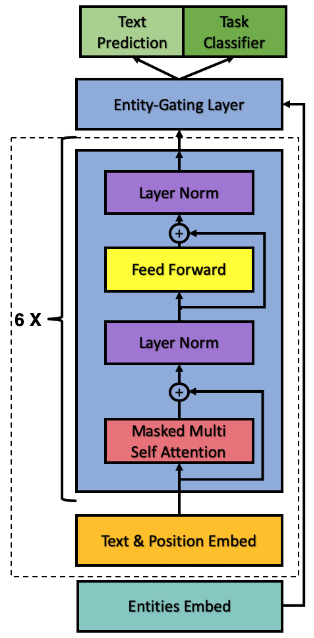
\includegraphics[scale=0.5]{gambar/DistilledGPT2Architecture.png}
  \caption{Arsitektur DistilGPT2}
  \label{fig:distilgpt2Architecture}
\end{figure}

Untuk dapat menghubungkan antara DistilGPT2 Model dan program DISC yang menggunakan Titian, penelitian ini akan memanfaatkan FastAPI. FastAPI adalah kerangka kerja web Python yang dikenal dengan kinerja tinggi, kemudahan pengembangan, dan otomatisasi pembuatan dokumentasi API. Dibangun di atas Python 3.6+ yang mendukung asynchronous programming, FastAPI dapat menangani banyak permintaan dengan cepat. Kerangka kerja ini menggunakan teknologi seperti Starlette dan Pydantic untuk memastikan penanganan permintaan HTTP yang efisien dan validasi data yang kuat [17]. Hingga kini FastAPI telah banyak dimanfaatkan untuk keperluan machine learning dan data science dan terbukti 45% jauh lebih baik dibandingkan dengan Flask [18]. Flask adalah framework web Python yang ringan dan fleksibel yang menekankan kesederhanaan dan kemampuan untuk diperluas. Ini menyediakan fitur dasar untuk pengembangan web dan memungkinkan pengembang memilih dan mengintegrasikan ekstensi berdasarkan kebutuhan proyek mereka [19].

DistilGPT2 Model yang ditanamkan ke dalam FastAPI kemudian akan di-deploy menggunakan Amazon Web Service (AWS) EC2. AWS adalah platform komputasi awan yang dikelola oleh Amazon. AWS menyediakan berbagai layanan komputasi, penyimpanan, database, jaringan, dan lainnya yang dapat digunakan oleh perusahaan dan pengembang untuk menjalankan aplikasi mereka di lingkungan awan. Amazon EC2 adalah salah satu layanan inti di AWS yang memungkinkan pengguna untuk menyewa mesin virtual (instance) di cloud. Pengguna dapat memilih berbagai jenis instance yang sesuai dengan kebutuhan mereka, seperti instance berkinerja tinggi, instance berbasis GPU, atau instance berbiaya rendah. AWS EC2 memungkinkan pengguna untuk dengan cepat meluncurkan, mengelola, dan menghentikan instance sesuai kebutuhan, sehingga mereka dapat mengskalakan aplikasi mereka sesuai dengan permintaan dan menghemat biaya saat instance tidak digunakan [20]. Dibandingkan dengan kompetitornya, AWS EC2 menawarkan solusi yang lebih baik di mana pengguna dapat memiliki kesempatan untuk memilih fitur yang diinginkan sesuai kebutuhan [21].

Pengembangan sistem akan menggunakan 2 bahasa pemrograman. Pada proses training awal model dan pembuatan FastAPI, bahasa pemrograman yang akan digunakan adalah Python. Sedangkan pada pembuatan sistem yang akan mengonsumsi FastAPI, bahasa pemrograman yang akan digunakan adalah Scala. Python dipilih untuk proses training awal model dan pembuatan FastAPI karena memiliki sintaksis yang mudah dipahami, ekosistem yang kaya, serta banyak library dan framework yang mendukung pengembangan aplikasi machine learning dan web termasuk HuggingFace. Kelebihan Python dalam kesederhanaan dan kemudahan penggunaan membuatnya menjadi pilihan utama dalam fase awal pengembangan [22]. Sementara itu, Scala dipilih untuk pembuatan sistem yang mengonsumsi FastAPI karena Scala menawarkan keunggulan dalam hal konkurensi dan eksekusi paralel, yang dapat meningkatkan kinerja sistem secara signifikan. Pemilihan Scala juga didorong oleh keandalan dan ekosistem yang mapan, terutama dalam pengembangan aplikasi berukuran besar [23]. Dibandingkan dengan Java pada bidang Natural Language Processing (NLP), Scala dianggap lebih unggul karena ekosistemnya yang lebih modern dan fitur-fitur fungsional yang dapat mempermudah pengembangan aplikasi NLP [24]. Scala memungkinkan penggunaan paradigma fungsional yang mendukung pemrosesan data kompleks dan manipulasi struktur data dengan lebih efisien, sehingga menjadi pilihan yang tepat untuk tugas-tugas kompleks dalam NLP [25].
